\section{The Structural Conditions of Corrigibility}
\label{sec:tests}

We define corrigibility as the existence of specific mechanical capabilities that allow the subjects of a system to maintain control over it. Digital Public Infrastructure cannot rely on intent or policy to guarantee this property; it requires a specific architecture.

These capabilities form a hierarchy of defense. If a system lacks any single capability, the feedback loop breaks. Such a system becomes structurally indistinguishable from a monopoly exercising absolute control.

\subsection{Test 1: EXIT (Reversibility of Participation)}

The foundational condition of any corrigible system is the \textbf{Reversibility of Participation}. Irrevocable consent functions structurally as conscription. For an infrastructure to operate as a public utility rather than a coercive instrument, users must possess the capacity to withdraw from it without incurring disproportionate penalty or material exclusion.

In practice, many systems operate as a ratchet. They are easy to enter but functional imperatives make them impossible to leave. \textbf{Aadhaar} exemplifies this failure: opting out results in exclusion from banking, food rations, and mobile connectivity. When a system becomes a prerequisite for existence, refusal acts as self-immolation rather than feedback. \textbf{UPI} partially mitigates this because cash remains legal tender, but network effects increasingly marginalize non-participants. \textbf{Linux}, by contrast, imposes no survival penalty: a user can migrate to BSD or Windows without losing access to essential services.

From a cybernetic perspective, EXIT constitutes the primary negative feedback loop. Blocking this channel silences the user's error signal. This blockade overloads the political layer with demands that the technical layer has suppressed.

This dynamic was formalized by Hirschman \citep{hirschman1970} in his analysis of organizational decline. Hirschman distinguished two correction mechanisms: exit (withdrawal from participation) and voice (attempts to change the system from within). His central finding is that these mechanisms exist in productive tension, not as substitutes.

Exit, in Hirschman's formulation, is ``neat,'' ``impersonal,'' and ``indirect'': one either exits or one does not. This binary quality makes exit a high-bandwidth error signal. When users leave, the system receives unambiguous information that something has failed. Voice, by contrast, is costly and conditioned on the influence and bargaining power that participants can bring to bear. Voice is gradual, political, and requires sustained effort.

Critically, Hirschman demonstrated that exit without voice produces abandonment rather than correction: quality-conscious users flee rather than fight. But voice without exit produces capture: complaints become cosmetic (see Section~\ref{subsec:grievance}) because the system faces no credible threat of user departure. The effectiveness of voice depends on the credibility of exit.

This framework illuminates why mandatory enrollment is structurally pathological. By eliminating exit, a system does not merely suppress one feedback channel. It degrades voice itself. When citizens cannot leave, their complaints lack credibility. The operator can absorb infinite grievance without modifying system behavior ($\partial S / \partial G = 0$). Hirschman's insight formalizes what cybernetics predicts: blocking the error signal does not eliminate the error; it eliminates the system's capacity to respond.

\subsection{Test 2: CODE (Inspectability of Logic)}

Users who cannot leave a system must possess the ability to inspect it. \textbf{Inspectability of Logic} requires that the rules determining outcomes are visible to those they govern. Power in a digital system resides in execution. Lessig \citep{lessig2006} established that software architecture functions as regulation: code ``determines what people can or cannot do in the first place,'' unlike legal regulation which sets rules for behavior and retroactively punishes non-compliance. This is regulation without appeal. If the execution path remains hidden, that power is absolute; it is not merely unaccountable but structurally unobservable to those it governs.

Transparency specifications or open standards are insufficient if the executing artifact remains a black box. \textbf{Aadhaar's} CIDR (Central Identities Data Repository) is proprietary: the matching algorithm that determines identity cannot be examined. \textbf{UPI} publishes API specifications, but the NPCI switching logic remains closed. \textbf{Let's Encrypt} demonstrates the alternative: its CA software is fully open source, allowing anyone to audit the certificate issuance logic that secures web traffic. For learned systems, the challenge intensifies. \textbf{Llama} publishes inference weights but withholds training data composition and RLHF preferences. This is spec-as-source: you can run the model but cannot understand why it produces specific outputs.

\subsection{Test 3: AUDIT (Independent Verification)}

While inspection enables understanding, \textbf{Independent Verification} enables truth. This functions as the sensor in the cybernetic feedback loop. A system is verifiable only if external, permissionless actors can test its behavior, measure its error rates, and document its failure modes within production environments.

Incorrigible systems typically capture this function. \textbf{UPI} permits RBI regulatory audits, but transaction-level verification requires NPCI authorization; independent researchers cannot measure failure rates or dispute resolution times. \textbf{Open-weights AI models} (Llama, Qwen, DeepSeek) selectively publish red-teaming results while blocking independent adversarial testing at scale. \textbf{Bitcoin} provides the counter-model: every transaction is independently verifiable by any node, and consensus is cryptographic proof. Similarly, \textbf{Let's Encrypt} publishes Certificate Transparency logs, making every issued certificate publicly auditable in real time.

\subsection{Test 4: GOVERN (Constitutive Constraint)}

Verification identifies the error, while \textbf{Constitutive Constraint} enforces the correction. This framework distinguishes structural governance from administrative functions like consultation, multi-stakeholder meetings, or feedback forms.

Governance exists only when binding constraints limit system behavior in ways the operator cannot override. \textbf{Aadhaar} is governed by UIDAI fiat: the same entity that operates the system sets its rules. \textbf{UPI} has NPCI governance, but NPCI is majority-owned by participating banks, creating structural conflicts. \textbf{Let's Encrypt} shows what binding constraint looks like: the ISRG charter legally binds the organization to its public benefit mission, with community board representation. \textbf{Bitcoin's} BIP process demonstrates governance through proven fork history; contentious changes have been rejected by the network, proving the community can override developer intent. \textbf{PostgreSQL's} contributor agreement prevents any single entity from capturing the project.

\subsubsection{The Post-Execution Fallacy}
A critical failure in modern policy involves relying on exogenous or post-hoc remedies to substitute for structural constraints. Mechanisms such as courts, ombudsmen, and grievance redressal officers operate on ``bureaucratic time,'' measured in months or years. Infrastructure operates on ``digital time,'' measured in milliseconds. A system that executes a harmful action, such as wrongful deletion of a beneficiary, and relies on a court order to reverse it six months later is structurally ungoverned for that duration. True governance must function within the system's execution loop to block prohibited states before they manifest.

Consequently, claims of governance must be evidentiary rather than declarative. They require a signed cryptographic chain of custody linking the operator's authority to an external, non-overrideable instrument.

\subsection{Test 5: FORK (Independent Reproduction)}

The ultimate check on power is the ability to recreate it. \textbf{Independent Reproduction} determines whether the ecosystem allows the infrastructure itself to be separated from its current steward. This requirement distinguishes structural resilience from simple market competition.

The existence of competitors, such as choosing between two proprietary cloud providers, provides an ``Exit'' option but not a ``Fork.'' Shifting providers allows a user to escape a specific operator, but it forces them to abandon their history, identity, and operational logic. This action is substitution, not reproduction.

A system passes the FORK test only if the community possesses the legal rights, technical artifacts, and economic means to spawn a functionally equivalent instance. \textbf{Aadhaar} fails completely: no entity outside UIDAI can reproduce the identity infrastructure. \textbf{OpenSearch} demonstrates what successful forking looks like. When Elastic changed its license, AWS forked Elasticsearch and the community continued development independently. \textbf{Linux} has been forked thousands of times (Android, Chrome OS, countless distributions). \textbf{Llama} presents partial forkability: anyone can run the weights, but reproducing the training requires resources only a handful of companies possess. If Meta abandoned Llama tomorrow, the community could not recreate it.

\begin{table}[htbp]
\centering
\begin{tabular}{@{}llll@{}}
\toprule
\textbf{System} & \textbf{EXIT} & \textbf{FORK} & \textbf{Structural Reality} \\
\midrule
Cloudflare & PASS (Market) & FAIL & Can switch to Fastly (Exit), cannot reproduce (Proprietary) \\
AWS & PASS (Market) & FAIL & Can migrate to Azure, logic/state locked (Ecosystem capture) \\
Aadhaar & FAIL (Mandatory) & FAIL & Cannot refuse (Legal), cannot reproduce (Total capture) \\
Linux & PASS & PASS & Can leave, can reproduce/fork (Corrigible infrastructure) \\
Llama & PASS & PARTIAL & Can refuse, can run weights, cannot reproduce training \\
\bottomrule
\end{tabular}
\caption{Differentiation between Exit (Substitution) and Fork (Reproduction)}
\end{table}

\subsection{The Topology of Necessity}

Five tests describe the anatomy of a stable control loop rather than a random assortment of normative virtues (see Figure~\ref{fig:topology}).

\begin{itemize}[noitemsep,topsep=0pt]
    \item \textbf{EXIT} provides the Error Signal.
    \item \textbf{AUDIT} acts as the Sensor.
    \item \textbf{CODE} ensures Transmission Clarity.
    \item \textbf{GOVERN} serves as the Actuator.
    \item \textbf{FORK} provides Selection Pressure over the entire loop.
\end{itemize}

Failure in any single dimension breaks the control loop at a specific physical point. The result is not partial infrastructure but \textbf{Open Loop Control}. An open-loop system executes directives without the capacity to sense deviation, interpret error, or apply corrective force.

Under conditions of human variety and environmental change, open-loop control is structurally unstable. Error accumulates without bound. Misalignment compounds. The system drifts toward failure.

Corrigibility is the structural precondition that closes the loop. Only when all five tests are satisfied does a system possess a complete feedback topology capable of detecting divergence, transmitting intelligible signals, executing correction, and replacing failed control logic when necessary. Without this closure, stability is mathematically and operationally impossible.

\begin{figure}[H]
\centering
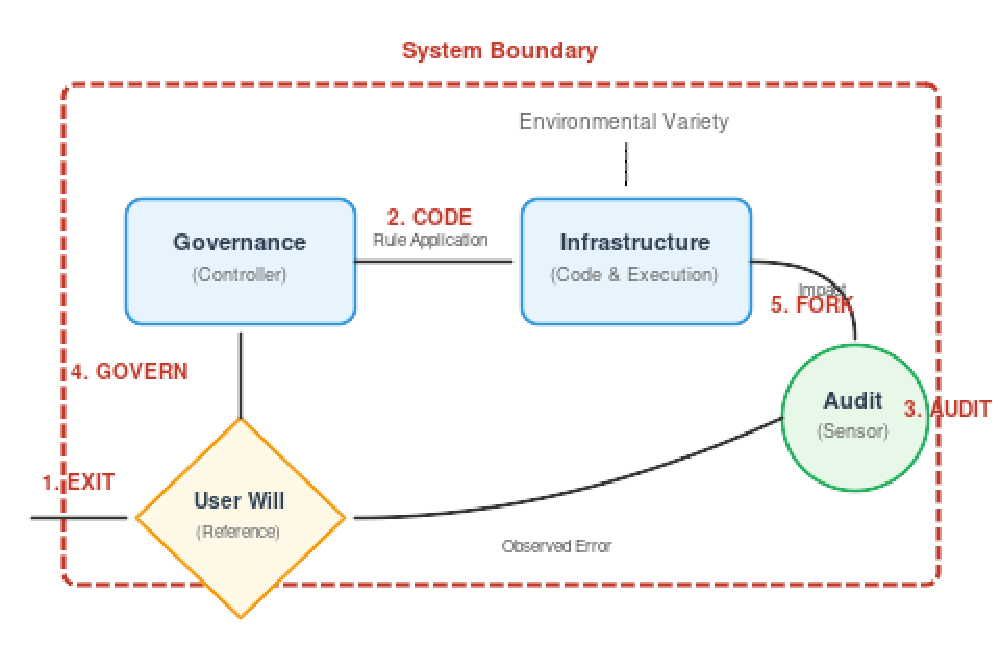
\includegraphics[width=0.75\textwidth]{figures/topology-of-necessity.pdf}
\caption{\textbf{Topology of Necessity.} Each corrigibility test corresponds to a breakage point in the feedback control loop.}
\label{fig:topology}
\end{figure}

\begin{figure}[H]
\centering
\begin{tikzpicture}[scale=0.85,
    tradition/.style={rectangle, rounded corners, draw=gray, fill=gray!10, minimum width=2.4cm, minimum height=0.7cm, font=\small},
    test/.style={rectangle, rounded corners, draw=#1, fill=#1!15, minimum width=1.5cm, minimum height=0.6cm, font=\small\bfseries},
    arrow/.style={-{Stealth[length=2mm]}, gray, thick}
]
% Three traditions at top
\node[tradition] (cyber) at (0,2.5) {Cybernetics};
\node[tradition] (commons) at (4,2.5) {Commons};
\node[tradition] (foss) at (8,2.5) {Free Software};

% Five tests at bottom
\node[test=exitcolor] (exit) at (0,0) {EXIT};
\node[test=codecolor] (code) at (2,0) {CODE};
\node[test=auditcolor] (audit) at (4,0) {AUDIT};
\node[test=governcolor] (govern) at (6,0) {GOVERN};
\node[test=forkcolor] (fork) at (8,0) {FORK};

% Connections - Cybernetics
\draw[arrow] (cyber.south) -- (exit.north);
\draw[arrow] (cyber.south) -- (audit.north west);

% Connections - Commons
\draw[arrow] (commons.south) -- (audit.north);
\draw[arrow] (commons.south) -- (govern.north);

% Connections - FOSS
\draw[arrow] (foss.south) -- (code.north east);
\draw[arrow] (foss.south) -- (fork.north);

% Labels
\node[font=\scriptsize, gray] at (4,-0.7) {All five tests required. Failure of any one disqualifies.};
\end{tikzpicture}
\caption{Five corrigibility tests derived from three independent theoretical traditions.}
\label{fig:framework}
\end{figure}

\subsection{Structural Symmetry of Power}

The five tests form a single power invariant, expressed across layers of control:

\begin{center}
\begin{tabular}{@{}lll@{}}
\toprule
\textbf{Layer} & \textbf{Test} & \textbf{Function (Cybernetic)} \\
\midrule
Individual & EXIT & Reversibility of participation \\
Logic & CODE & Inspectability of rules \\
Logic & AUDIT & Verifiability of error \\
System & GOVERN & Constraint on controller variance \\
Ecosystem & FORK & Selection pressure via reproduction \\
\bottomrule
\end{tabular}
\end{center}

Each test enforces the same principle: \textit{No actor exercising power may be the sole judge of its continuation, scope, or correction.}

A system without EXIT is coercive. A system without GOVERN is arbitrary. A system without FORK is captive.

\subsection{Layer-Decomposed Evaluation}
\label{subsec:layers}

Complex infrastructure frequently stratifies into distinct functional layers, each with independent governance, transparency, and reproducibility properties. The five tests must be applied to each layer separately when:

\begin{enumerate}[noitemsep,topsep=0pt]
    \item Different entities control different layers (protocol versus implementation versus trust framework)
    \item Transparency varies across layers (open protocol, closed switching logic)
    \item Forkability differs by layer (code is forkable, network effects are not)
\end{enumerate}

\subsubsection{Propagation Rule}

A system that passes a test at one layer but fails at another does not achieve ``partial'' compliance. It fails the test. The evaluation proceeds from the layer closest to user impact upward; failure at any layer propagates to the whole.

Formally: Let $L_1, L_2, \ldots, L_n$ be the layers of a system, ordered by proximity to user impact. For test $T$:

\begin{equation}
T_{\text{system}} = \bigwedge_{i=1}^{n} T(L_i)
\end{equation}

The system passes $T$ if and only if every layer passes $T$.

\subsubsection{Application to Identity Infrastructure}

\begin{table}[htbp]
\centering
\small
\begin{tabular}{@{}llp{5cm}@{}}
\toprule
\textbf{Layer} & \textbf{Example Components} & \textbf{Typical Failure Mode} \\
\midrule
Protocol & W3C DID, VC Data Model & Often passes CODE \\
Implementation & Specific resolver, wallet software & May fail CODE (proprietary) \\
Credential & Issuer policies, attribute schemas & Often fails GOVERN (unilateral issuer) \\
Trust & Relying party acceptance, trusted lists & Often fails FORK (cannot reproduce acceptance) \\
\bottomrule
\end{tabular}
\caption{Identity infrastructure layer decomposition}
\label{tab:identity_layers}
\end{table}

The UPI payment rail exhibits similar layering: the protocol specification (NPCI-published) passes CODE at the protocol layer, but the switching logic (NPCI-operated) fails CODE at the implementation layer. Since the implementation layer is closer to user impact, the system fails CODE.

\subsubsection{The Weakest-Layer Principle}

This propagation rule has a counterintuitive but structurally necessary consequence: a system's corrigibility status equals its weakest layer across any test dimension. Strength at one layer cannot compensate for failure at another.

This principle prevents a common evasion: claiming corrigibility by publishing peripheral artifacts while retaining control over the layers that determine outcomes. Open-washing (Section~\ref{subsec:openwashing}) typically exploits layer confusion. Releasing SDKs (passing CODE at the interface layer) while keeping core logic proprietary (failing CODE at the execution layer) does not produce partial corrigibility. It produces total failure at the execution layer, which propagates to the system determination.